\documentclass[user_manual.tex]{subfiles}
\begin{document}
\chapter{Puesta en marcha}
En este capitulo se explicara de forma concisa el uso y funcionamiento del robot de forma practica, así como mostrar alternativas para el uso de los nodos sin contar con el hardware para realizar pruebas de funcionamiento. Como primera instancia se ilustrara la forma de conexión entre las dos computadoras (las cuales fueron mencionadas en el capitulo 3 primeros pasos), así como la conexión de esta con el hardware de Justina.

\section{Conexión linux-windows}
Como se explico en el capitulo 3 para hacer la comunicación entre las dos computadoras se requiere una conexión punto a punto, la cual está explicada en el apendice B Software.\\

En esta sección se explicará como llevar a cabo la comunicación entre ambas computadoras para así poder utilizar el reconocimiento de voz y la generación de voz; las cuales son utilizadas en diferentes pruebas.\\

Para establecer la conexión entre las dos computadoras se debe usar un cable ethernet.\\

Antes de empezar se debe verificar que la computadora con windows cuente con una ip fija para poder comunicarse con la computadora con ubuntu. La ip se muestra a continuación:

\begin{center}
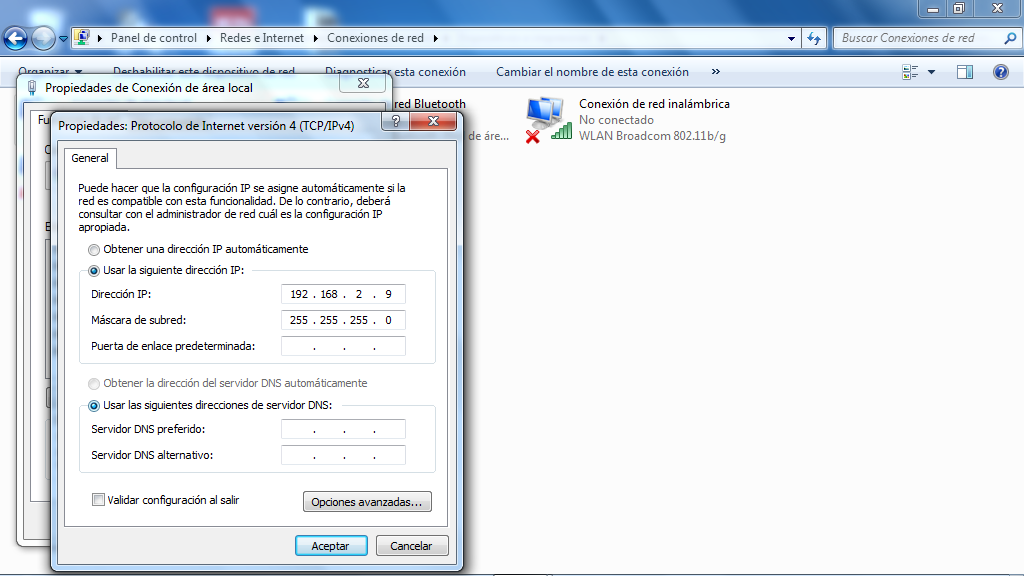
\includegraphics[width=0.8\textwidth]{Figures/Puesta_marcha/red.png}
\captionof{figure}{Ip fija}
\end{center}


\subsection{Comunicación de ubuntu}

Al conectar por medio de cable ethernet la computadora plateada a la de ubuntu deberá aparecer una red llamada $"Plateada"$ a la cual se debe conectar la computadora con ubuntu para empezar a establecer una comunicación.


\begin{center}
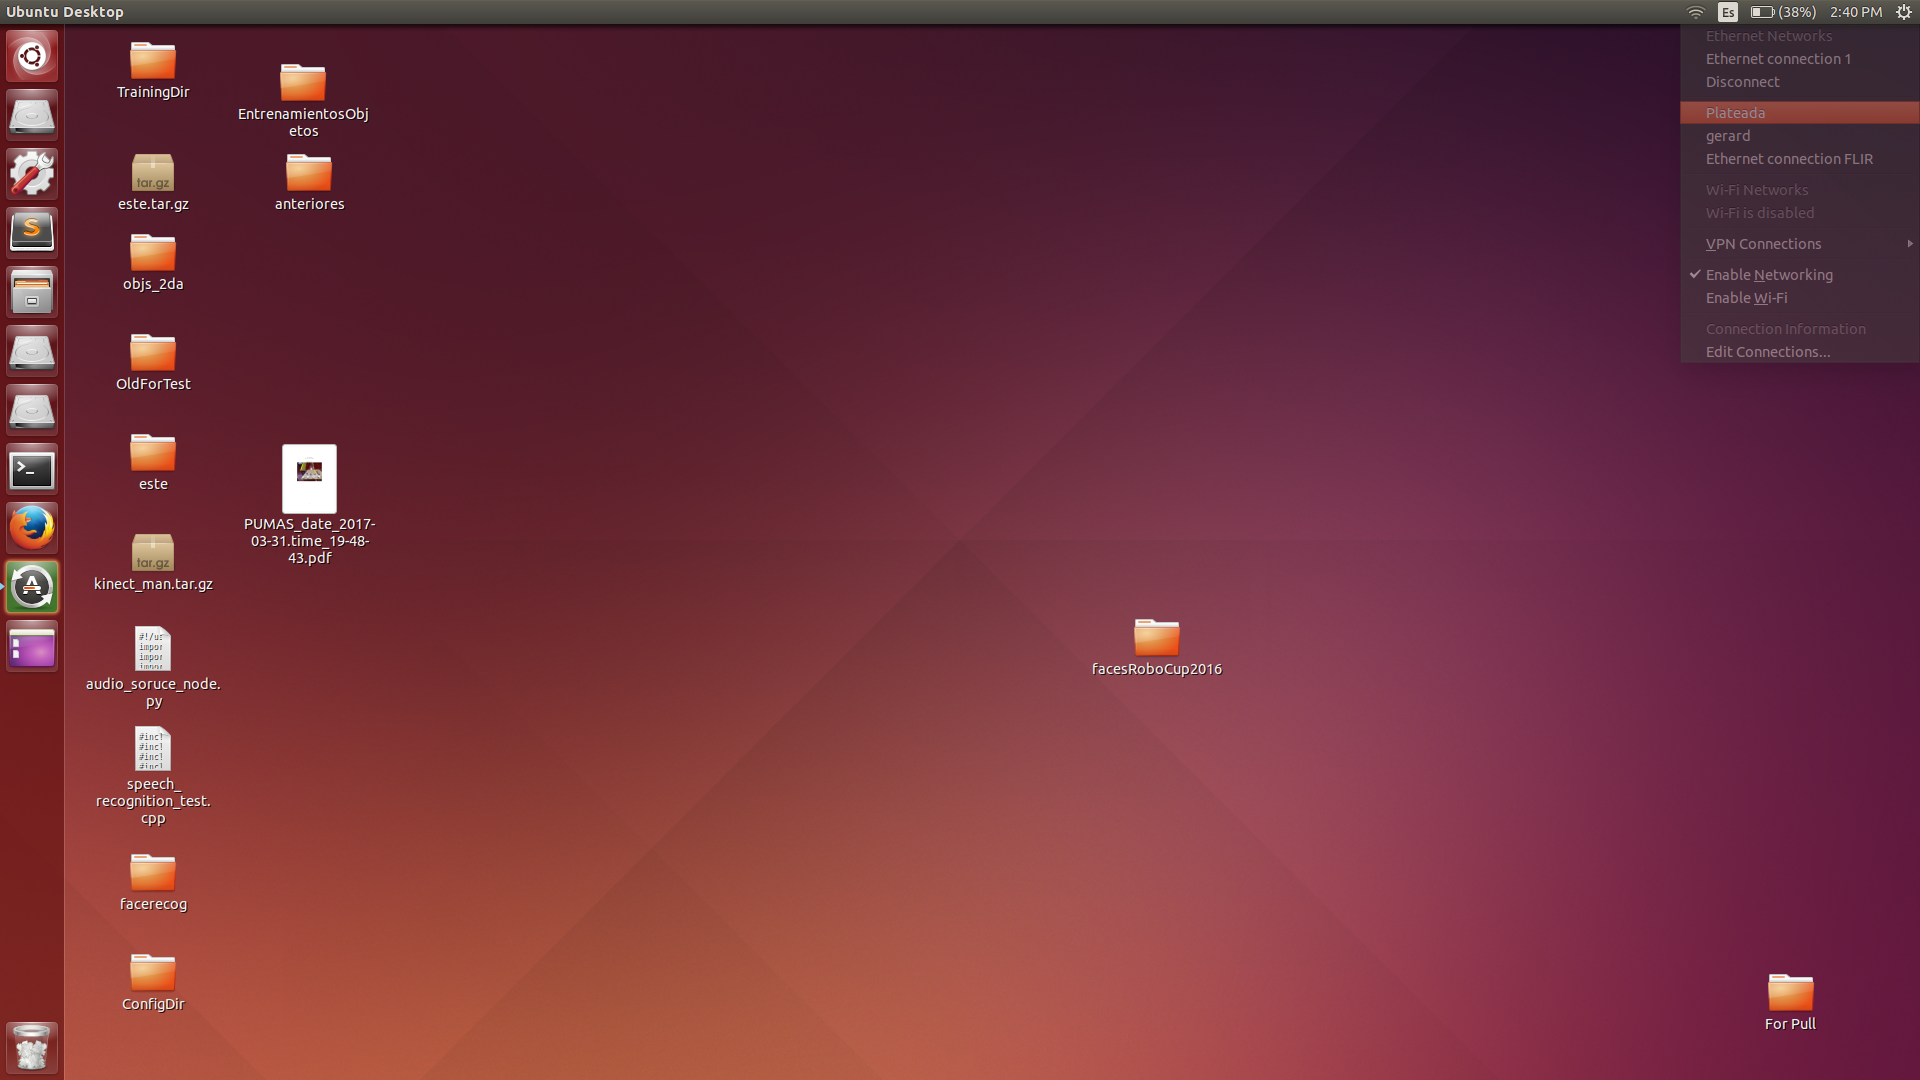
\includegraphics[width=0.9\textwidth]{Figures/Puesta_marcha/Red_plateada.png}
\captionof{figure}{Red Plateada}
\end{center}



\subsection{Configuración de Blackboard en windows}

El programa empleado para establecer la comunicación de los programas sp\_rec y sp\_gen con linux es blackboard. La computadora que se tomara como ejemplo para la conexión es la llamada ''plateada''.\\

La forma de configurar Blackboar para su uso con la computadora con linux es la siguiente:\\

1. Ejecutar el programa blackboard, del cual se encuentra un acceso directo en el escritorio de la plateada:

%Figura
\begin{center}
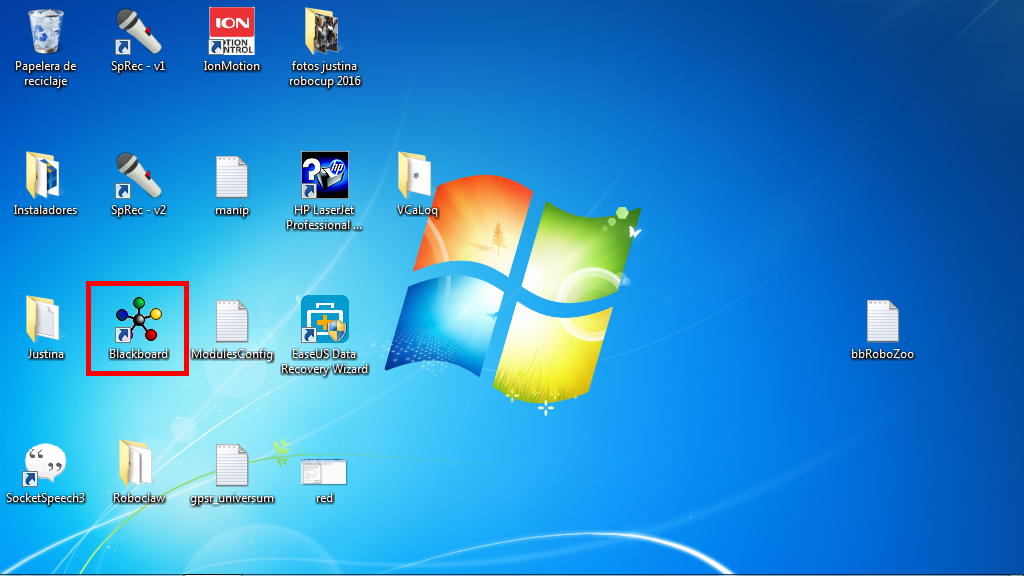
\includegraphics[width=0.65\textwidth]{Figures/Puesta_marcha/Abrir_Bb.png}
\captionof{figure}{Blackboard en el escritorio}
\end{center}

2. Al abrir Blackboard se debe selecciónar el archivo de configuración y cargarlo a Blackboard; ésto se hace de la siguiente forma:

%Figura
\begin{center}
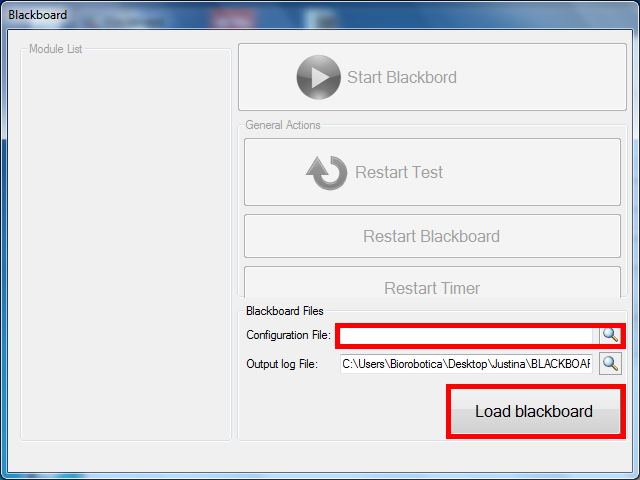
\includegraphics[width=0.65\textwidth]{Figures/Puesta_marcha/Config_file.png}
\captionof{figure}{Selección del archivo}
\end{center}

El archivo se encuentra en el directorio $"Aqui va el directorio"$.\\

3. Una vez cargado el archivo de configuración se debe presionar el boton $ "Start Blackboard"$.

%Figura
\begin{center}
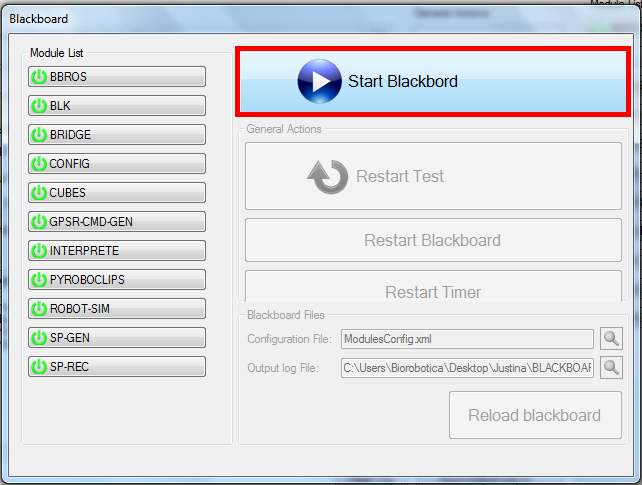
\includegraphics[width=0.65\textwidth]{Figures/Puesta_marcha/Activar_Bb.png}
\captionof{figure}{Acivación de blackboard}
\end{center}


4. Despues de presionar $"Start Blackboard"$ aparecera a la izquierda una lista de los modulos existentes que fueron configurados para Blackboard. Los modulos que aparecen con una palomita son los modulos habilitados y los que tienen un tache son los modulos deshabilitados.

%Figura
\begin{center}
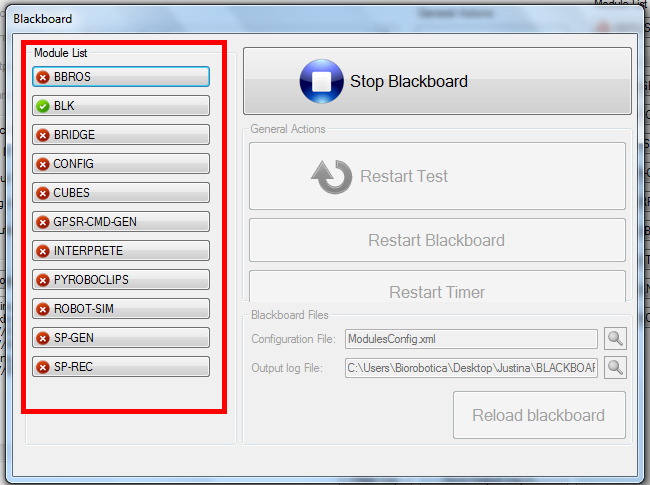
\includegraphics[width=0.65\textwidth]{Figures/Puesta_marcha/Modulos_Bb.png}
\captionof{figure}{Modulos en blackboard}
\end{center}

Para poner en marcha a Justina se necesitan los siguientes modulos:

\begin{itemize}
\item BLK
\item BRIDGE
\item SP-GEN
\item SP-REC
\end{itemize}

El modulos $"BRIDGE"$ sólo puede ser habilitado cuando la computadora con ubuntu se encuentra conectada al hardware de Justina, de lo contrario no se podra habilitar.\\

Los modulos SP-GEN y SP-REC podran ser habilitados abriendo los respectivos programas los cuales se encuentran también en el escritorio.

%Figura
\begin{center}
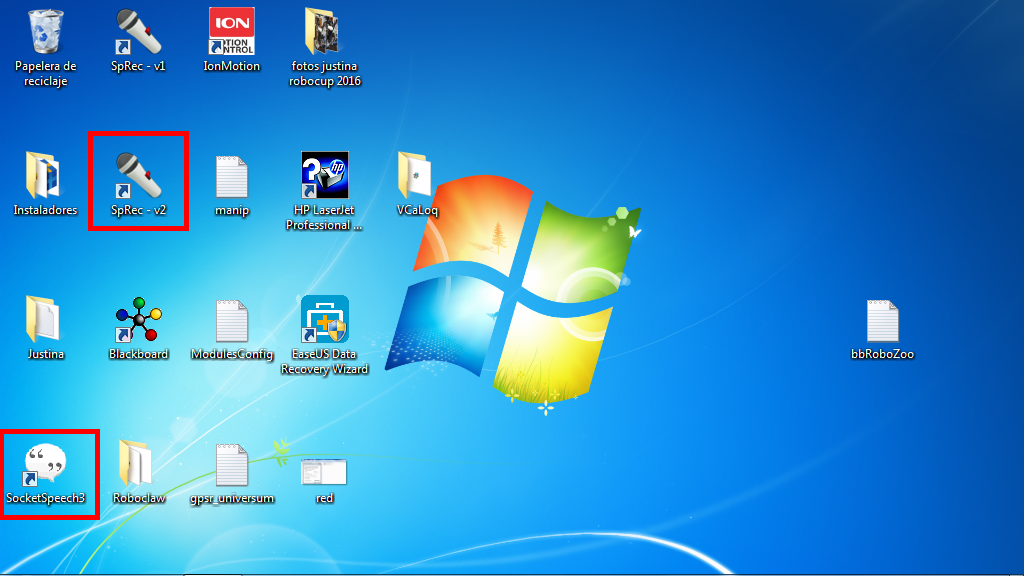
\includegraphics[width=0.65\textwidth]{Figures/Puesta_marcha/SpRec_SpGen.png}
\captionof{figure}{SPREC y SPGEN en el escritorio}
\end{center}


\subsubsection{SP-GEN}

Para habilitar este programa en blackboard basta simplemente con ejecutarlo. En este programa se puede seleccionar la voz que tendrá Justina. Se tiene la voz de Susan por defecto, ya que es la utilizada comunmente.

\begin{figure}[H]
\centering
\subfigure[SPGEN]{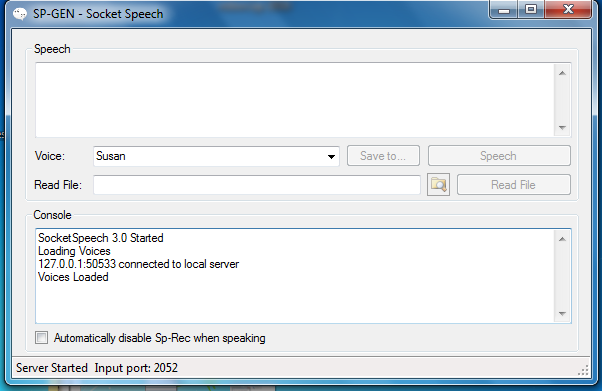
\includegraphics[width=80mm]{Figures/Puesta_marcha/SPGEN.png}}
\subfigure[Otras voces]{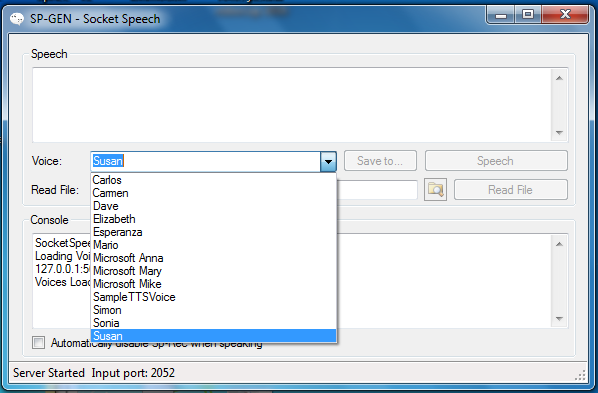
\includegraphics[width=80mm]{Figures/Puesta_marcha/SPGEN1.png}}
\caption{Legos.} \label{fig:SP-GEN}
\end{figure}

\subsubsection{SP-REC}

Para habilitar SP-REC en blackboard se deben seguir ciertos pasos los cuales se muestran a continuación:

1. Al ejecutar el programa aparecera la siguiente ventana, donde se debe seleccionar el archivo de gramatica que se desea utilizar.

%Figura
\begin{center}
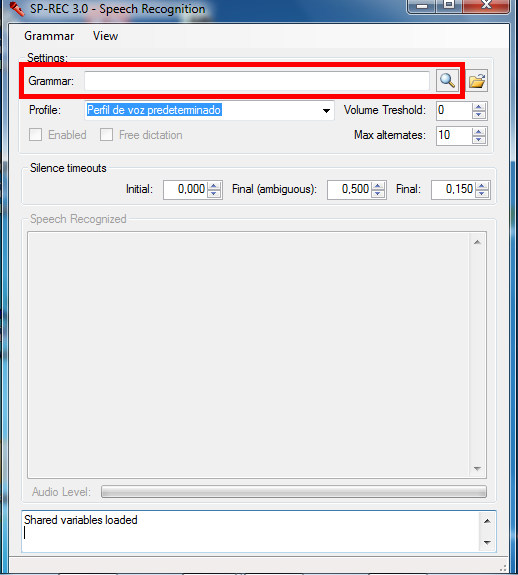
\includegraphics[width=0.65\textwidth]{Figures/Puesta_marcha/SPREC_gram.png}
\captionof{figure}{SPREC}
\end{center}

Como ejemplo se utiliza el archivo $"followme"$ el cual se utiliza comunmente.

%Figura
\begin{center}
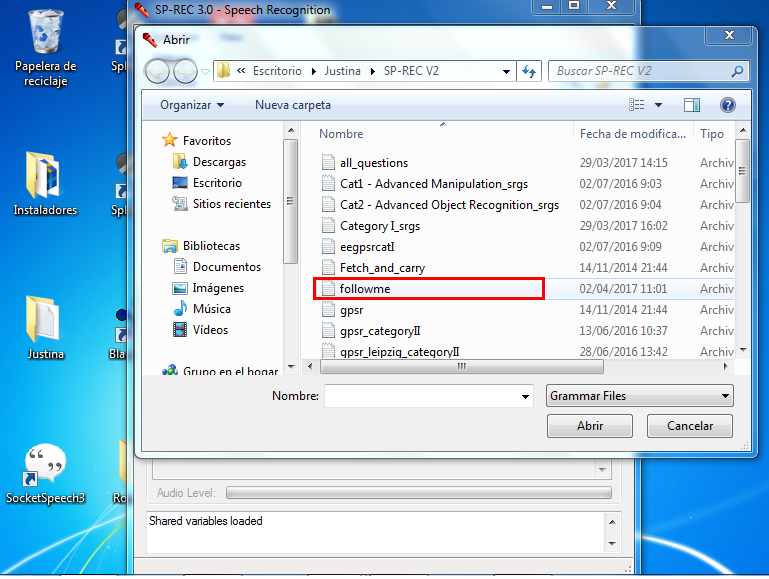
\includegraphics[width=0.65\textwidth]{Figures/Puesta_marcha/SPREC_file.png}
\captionof{figure}{Selección de la gramatica}
\end{center}

2. Despues de seleccionar el archivo es necesario cargarlo al programa SP-REC.

%Figura
\begin{center}
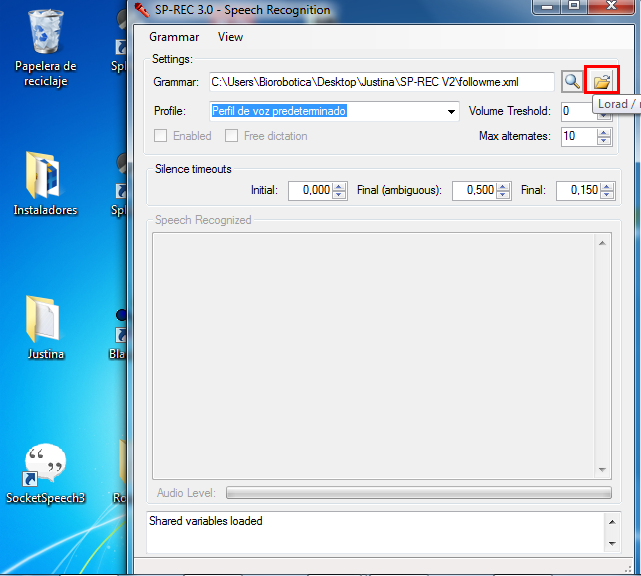
\includegraphics[width=0.65\textwidth]{Figures/Puesta_marcha/SPREC_load.png}
\captionof{figure}{Carga de la gramatica en SPREC}
\end{center}

3. Por ultimo se debe marcar la casilla $"Enabled"$ para habilitar el modulo en Blackboard.

%Figura
\begin{center}
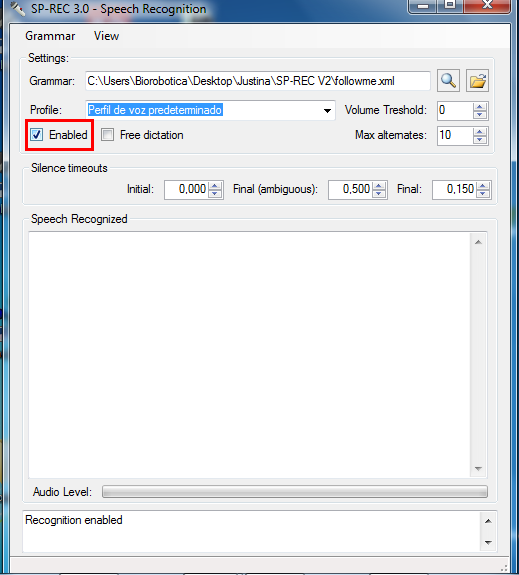
\includegraphics[width=0.65\textwidth]{Figures/Puesta_marcha/SPREC_enable.png}
\captionof{figure}{Habilitación de la gramatica}
\end{center}

Una vez que se siguieron los pasos anteriores aparecerán sus modulos habilitados en la lista de blackboard.

%Figura
\begin{center}
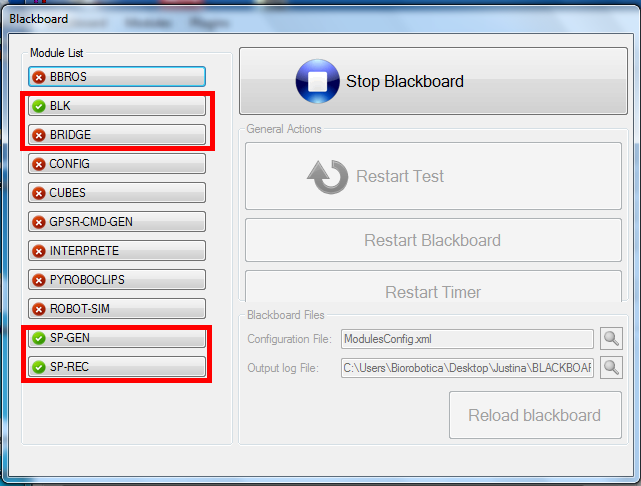
\includegraphics[width=0.65\textwidth]{Figures/Puesta_marcha/Modulos_activados.png}
\captionof{figure}{Modulos habilitados}
\end{center}

Como se menciono anteriormente para que el modulo $"BRIDGE"$ sea habilitado la computadora con ubuntu debe estar conectada al hardware de Justina además de estar conectada por cable ethernet a la computadora con windows.

\section{Rviz}
Para probar el funcionamiento del hardware y software de Justina se puede utilizar Rviz y la GUI. Para ejecutar estos programas se puede hacer uso de diferentes launche y run de ros.\\

Rviz es una herramienta de visualización 3D de ROS. Es un visualizador de datos muy util y completo, pero hay varias cosas que se deben considerar.

\subsubsection{Frames de coordenadas}

Hay dos frames de coordenadas importantes:\\

  1.  El fixed frame. Es el sistema de coordenadas que tomaremos como referencia para mostrar todos lo datos. Aparece en la parte izquierda en Global options. Se debe asignar a un punto estático como el mundo o el mapa. En caso de no tenerlo se puede asignar al de odometría. No se debe asignar a un frame en movimiento, como la base de un robot.\\
  
  2.  El target frame.  Es el sistema de coordenadas que asi se asigna a la vista. Éste sí se puede poner a la base del robot, por ejemplo. Se pueden tener distintas vistas y así ir cambiando de una a otra en función de lo que se desea ver.

\subsubsection{Modo de operación}

Existen diversos modos de operación. Se pueden seleccionar en la parte superior. Por defecto está en interactuar y podemos también mover la cámara, seleccionar elementos (y ver sus valores, por ejemplo coordenadas de puntos), etc.

%Figura
\begin{center}
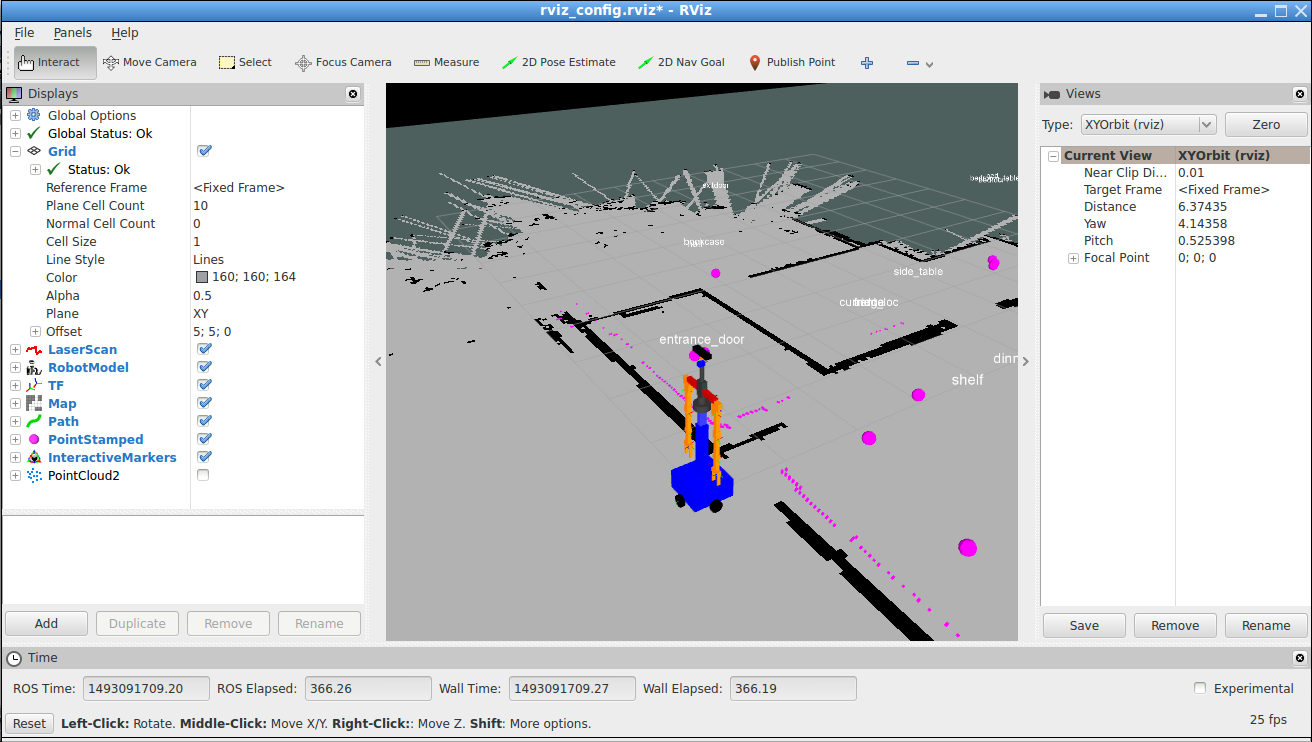
\includegraphics[width=0.9\textwidth]{Figures/Puesta_marcha/RViz.png}
\captionof{figure}{General}
\end{center}

\section{GUI}
GUI
\subsection{General}
Como su nombre lo indica, en la pestaña general se muestran los aspectos más generales, así como la manipulación de los actuadores del robot; para esto se cuenta con diferentes menus que ayudan de forma intuitiva al uso de estos

%Figura
\begin{center}
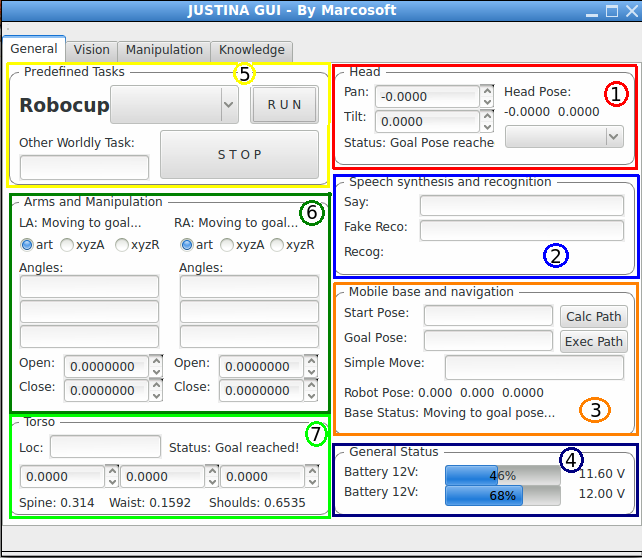
\includegraphics[width=0.65\textwidth]{Figures/Puesta_marcha/General.png}
\captionof{figure}{General}
\end{center}

\subsubsection{HEAD}

Este modulo cuenta con dos controles para el movimiento de inclinación y rotación de la cabeza.

\begin{table}[H]
\begin{center}
\begin{tabular}{|l|l|}%Define el número de columnas

\hline
\multicolumn{2}{|c|}{Head}\\ \hline
Tilt  & Con este control se hace el cambio de angulo de inclinación \\ \hline 
Pan   & Con este control se hace el cambio de angulo de rotación\\ \hline

\end{tabular}
\end{center}
\end{table}
%Fin de la tabla

%Figura
\begin{center}
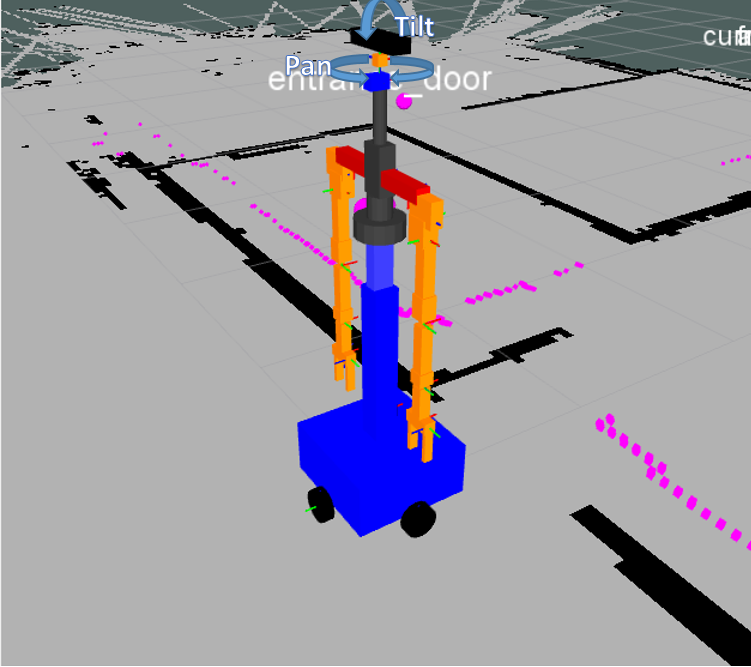
\includegraphics[width=0.45\textwidth]{Figures/Puesta_marcha/Tilt_pan.png}
\captionof{figure}{Movimientos tilt y pan}
\end{center}

\subsubsection{Speech synthesis and recognition}

\begin{table}[H]
\begin{center}
\begin{tabular}{|l|l|}%Define el número de columnas

\hline
\multicolumn{2}{|c|}{Speech synthesis and recognition} \\ \hline
Say        & Aquí se escribe lo que se quiere que diga Justina\\ \hline
Fake Recog & Aquí se escribe lo que se busca reconocer \\ \hline
Recog      & Aquí muestra se reconocio     \\ \hline


\end{tabular}
\end{center}
\end{table}
%Fin de la tabla

\subsubsection{Mobile base and navigation}

Este modulo sirve para m

\begin{table}[H]
\begin{center}
\begin{tabular}{|l|l|}%Define el número de columnas

\hline
\multicolumn{2}{|c|}{Mobile base and navigation}                                                   \\ \hline
Start pose      & Se igresa la posición actual de Justina o se puede ingresar el comando ''Robot" * \\ \hline
Goal pose       & Se ingresa el destino al cual se desea que avance a Justina **                     \\ \hline
Simple pose     & Se ingresan los valores de avance y ángulo que se quiere mover a Justina            \\ \hline
Robot Pose      & Muestra las coordenadas XY y el ángulo de Justina respecto a su posición inicial     \\ \hline
Base status     & Muestra el estado en el que se encuentra la base                                      \\ \hline
\end{tabular}
\end{center}
\end{table}
%Fin de la tabla

* El comando Robot es utilizado para que Justina tome como referencia su posición actual para calcular la ruta hacia su destino.\\

** Una vez indicado el destino de Justina, al presionar el boton ''Calc Path" se calcula la mejor ruta que Justina puede tomar para llegar a su destino. Cuando la ruta es calculada, al presionar el boton ''Exec Path" Justina avanza hacia su destino.



\subsubsection{General Status}

Este modulo está disponible tanto en las pruebas con el hardware como en la simulación. En las pruebas con el hardware muestra el valor de voltaje en las baterias y en la simulación muestra un valor fijo de voltaje.

\begin{table}[H]
\begin{center}
\begin{tabular}{|l|l|}%Define el número de columnas

\hline
\multicolumn{2}{|c|}{General Status} \\ \hline
Battery 12 volts  & Muestra el nivel de voltaje de las baterias  \\ \hline


\end{tabular}
\end{center}
\end{table}
%Fin de la tabla

\subsubsection{Predefined Tasks}

Este modulo no se encuentra disponible por el momento. 

\subsubsection{Arms and manipulation}

Este modulo de control funciona tanto en el hardware como en la simulación de Justina. La función de este modulo es controlar y manipular los brazos y gripers de Justina mediante comandos para los movimientos de los brazos y cambiando el valor de los controles para el ángulo de apertura de los gripers.

\begin{table}[H]
\begin{center}
\begin{tabular}{|l|l|l|}%Define el número de columnas

\hline
\multicolumn{3}{|c|}{Arms and manipulation}                                                         \\ \hline
\multirow{2}{3cm}{Left Arm}  &  LA:     & Muestra el estado del brazo                                \\ \cline{2-3}
                             &  Angles: & Se escribe la acción que se desea realizar con el brazo     \\ \cline{2-3}
                             &  Open:   & Control para abrir y cerrar el griper del brazo izquierdo    \\ \hline
\multirow{2}{3cm}{Right Arm} &  RA:     & Muestra el estado del brazo                                   \\ \cline{2-3}
                             &  Angles: & Se escribe la acción que se desea realizar con el brazo        \\ \cline{2-3}
                             &  Open:   & Control para abrir y cerrar el griper del brazo derecho         \\ \hline 
Close                        & \multicolumn{2}{|c|}{Este control no se encuentra activo para ningun brazo} \\ \hline
\end{tabular}
\end{center}
\end{table}
%Fin de la tabla

\subsubsection{Torso}

Esta función está disponible unicamente en la simulación, ya que no se ha implementado en las pruebas físicas de Justina.

\subsection{Vision}

%Figura
\begin{center}
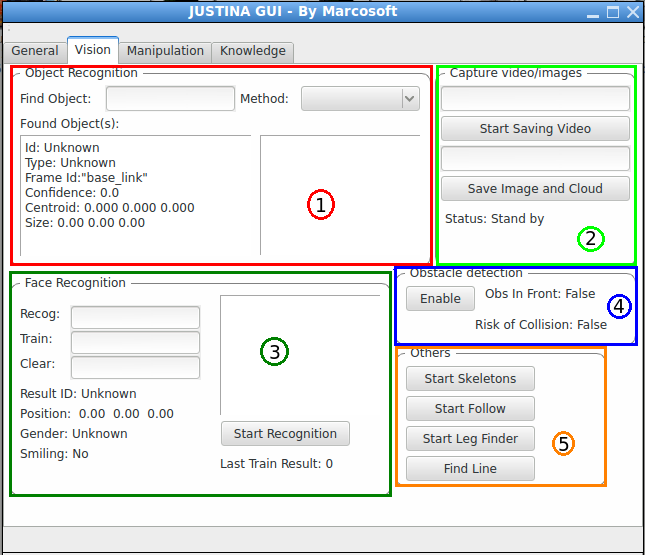
\includegraphics[width=0.65\textwidth]{Figures/Puesta_marcha/Vision.png}
\captionof{figure}{Vision}
\end{center}

\subsubsection{Object Recognition}

\begin{table}[H]
\begin{center}
\begin{tabular}{|l|l|l|}%Define el número de columnas

\hline
\multicolumn{3}{|c|}{Object Recognition}\\ \hline
Find Object:                         &\multicolumn{2}{|c|}{Se ingresa el nombre asociado al objeto que se desea encontrar}                                                         \\ \hline
Method:          					  &\multicolumn{2}{|c|}{Sólo existe un metodo para encontrar objetos}\\ \hline
\multirow{6}{3cm}{Found Object(s):}  &\multicolumn{2}{|c|}{Muestra los parametros del objeto a encontrar}\\ \cline{2-3}
                                     &  ID:         & Muestra el id del objeto  \\ \cline{2-3}
                                     &  Type:       &     \\ \cline{2-3}
                                     &  Frame Id:   & ''base\_link''\\ \cline{2-3} 
                                     &  Confidence: & 0.0   \\ \cline{2-3}
                                     &  Centroid:   & Muestra las coordenadas del objeto   \\ \cline{2-3}
                                     &  Size:       & Muestra las medidas del objeto   \\ \hline
\end{tabular}
\end{center}
\end{table}
%Fin de la tabla

Al ejecutar la busqueda se abre una nueva pestaña la cual muestra en tiempo real lo que es captado por la cámara; también se muestran etiquetas en los objetos reconocidos.

\subsubsection{Capture Video/Images}


\begin{table}[H]
\begin{center}
\begin{tabular}{|l|l|l|}%Define el número de columnas

\hline
\multicolumn{2}{|c|}{Capture Video/Images}\\ \hline
Start Saving Video    & Al presionar el botón se guada el archivo de vídeo  \\
                      &una vez ingresado el nombre en el espacio  \\ \hline
Save Image and Cloud  & Al presionar el botón se guarda la imagen una vez\\
					   & ingresado el nombre del archivo  \\ \hline


\end{tabular}
\end{center}
\end{table}
%Fin de la tabla




\subsubsection{Face Recognition}

\begin{table}[H]
\begin{center}
\begin{tabular}{|l|l|}%Define el número de columnas

\hline
\multicolumn{2}{|c|}{Face Recognition}\\ \hline
Recog:                  &\\ \hline
Train:                  &\\ \hline
Clear:                  &\\ \hline
Result ID:              &\\ \hline
Position:               &\\ \hline
Gender:                 &\\ \hline 
Smiling:                &\\ \hline
Start Recognizer        & Al presionar el botón se inicia el reconocimiento\\ \hline
Last Train Result:      &\\ \hline
\end{tabular}
\end{center}
\end{table}
%Fin de la tabla


\subsubsection{Obstacle Detection}

\begin{table}[H]
\begin{center}
\begin{tabular}{|l|l|}%Define el número de columnas

\hline
\multicolumn{2}{|c|}{Obstacle Detection}\\ \hline
Enable/Disable        & Al presionar el botón se cambía de estado  \\
                      & habilitando o deshabilitando la detección \\
                      & de obstaculos,  \\ \hline
Obs In Front:         & Muestra el estado True/False\\ \hline
                      & Muestra el estado para riesgo de colisión \\
Risk of Collision:    & True/False\\ \hline


\end{tabular}
\end{center}
\end{table}
%Fin de la tabla




\subsubsection{Others}

\begin{table}[H]
\begin{center}
\begin{tabular}{|l|l|}%Define el número de columnas

\hline
\multicolumn{2}{|c|}{Others}\\ \hline
Start Skeletons       & Al presionar el botón se cambía de estado  \\ \hline
Start Follow          & habilitando o deshabilitando la detección   \\ \hline
Start Leg Finder      & de obstaculos                                \\ \hline
Find Line             & Muestra el estado True/False                  \\ \hline

\end{tabular}
\end{center}
\end{table}
%Fin de la tabla




\subsection{Manipulation}

%Figura
\begin{center}
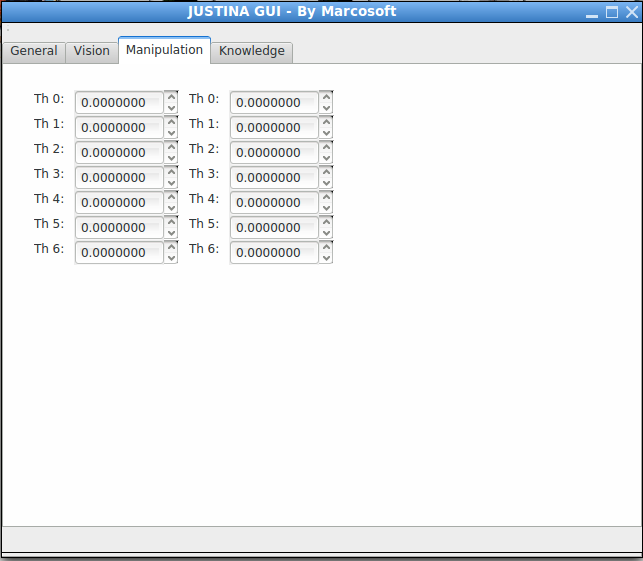
\includegraphics[width=0.65\textwidth]{Figures/Puesta_marcha/Manipulation.png}
\captionof{figure}{Manipulation}
\end{center}

\begin{table}[H]
\begin{center}
\begin{tabular}{|l|l|}%Define el número de columnas

\hline
\multicolumn{2}{|c|}{Manipulation}\\ \hline
   &  \\ \hline 
   & \\ \hline

\end{tabular}
\end{center}
\end{table}
%Fin de la tabla

\section{Knowledge}

\section{Pruebas}
\begin{minted}[
frame=lines,
framesep=1mm,
bgcolor=black,
baselinestretch=1.2
]{console}
 ~$ roslaunch surge_et_ambula justina.launch
\end{minted}
%$

 \begin{center}
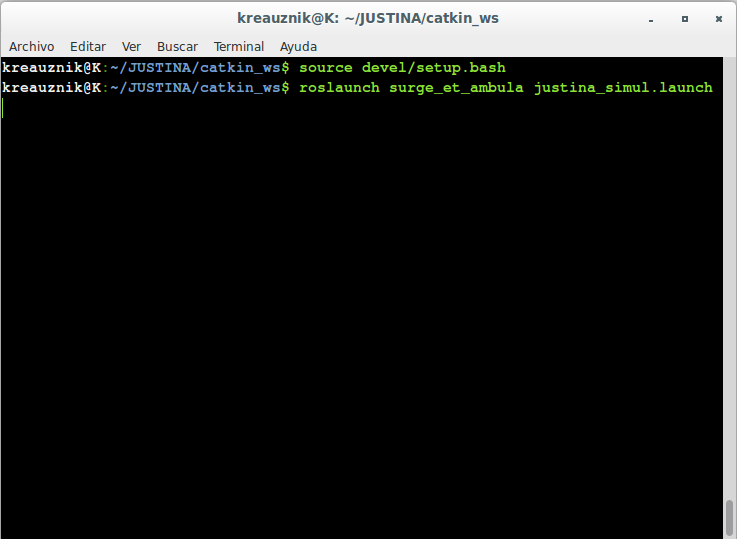
\includegraphics[width=0.73\textwidth]{Figures/PP/pp6.png}
\end{center}
\section{Simulación en el RViz y GUI de Justina}
Una alternativa para utilizar el software y hacer pruebas cuando no se cuenta con el hardware es utilizar la simulación de Rrviz y GUI, para esto se debe ejecutar el siguiente comando:\\

\begin{minted}[
frame=lines,
framesep=1mm,
bgcolor=black,
baselinestretch=1.2
]{console}
 ~$ roslaunch surge_et_ambula justina_simul.launch
\end{minted}
%$\\

Esto nos permite ocupar funciones del software de Justina, pero no es posible ocupar todas ya que algunas son dependientes de hardware y este es necesario para su correcto funcionamiento. Está opción para ocupar Rviz y GUI puede ocupar muchos recursos por lo que a continuación se dispodran algunas pruebas que pueden ser ejecutadas sin necesidad del hardware.


\end{document}